\chapter{Meridional characteristics of GWs excited by propagating tropopause depressions}
\label{sec:results3D}
3D simulations of the previous section focused on the analysis of zonal and vertical properties of stratospheric GWs using a 2D tropopause depression and a low grid resolution in meridional direction. However, in reality the shape of a tropopause depression varies meridionally and the PNJ is often not centered above the depression and entails meridional wind shear. Therefore, this section presents full 3D simulations with an identical resolution in streamwise and spanwise direction, a 3D tropopause depression and a zonal background wind with meridional shear $u_e(z,y)$. \\
Subsequent to Chapter \ref{sec:resultsQ3D}, it is the goal to address the sensitivity of NOGWs above tropopause depressions to meridional variations of the tropopause and stratospheric airflow by investigating the second research question
\begin{tcolorbox}[]
    (R2) How sensitive are NOGWs from propagating tropopause depressions to the depression's 3D shape and meridional variations of the stratospheric airflow?
\end{tcolorbox}
In addition, realistic simulations of the stratosphere facilitate the investigation of the third research question, which refers to the zonally elongated phase lines in the horizontal cross-sections of Figure \ref{fig:RF25_era5_horizonal}.
\begin{tcolorbox}[]
    (R3) Can NOGWs above propagating tropopause depressions explain the zonally elongated phase lines in ERA5 above the Southern Ocean?
    % the zonally elongated phase lines in the horizontal cross-sections of Figure \ref{fig:RF25_era5_horizonal}. 
    % long vertical wave lengths in vertical cross-section and elongated phase line in horizontal
\end{tcolorbox}
All simulations of this chapter have the same temporal resolution (dt$=\SI{60}{\second}$) as simulations of Chapter \ref{sec:resultsQ3D}, but the horizontal and vertical domain is adapted to (n$_z$,n$_y$,n$_x$)=(251,480,720) grid points with a resolution of (dz,dy,dx)=(\SI{300}{\meter},\SI{20}{\kilo\meter},\SI{20}{\kilo\meter}). Again, periodic boundaries are used streamwise, linear sponge layers are used spanwise and the exponential sponge layer described in the "lessons learned" of Section \ref{sec:linear-MWs} is used vertically.

Two processes lead to a meridional propagation of GWs. The first process is solely caused by the 3D shape of the obstacle and becomes relevant as soon as the obstacle's shape changes in spanwise direction. The flow is not only deflected vertically, but also horizontally (flow around the isolated obstacle), which can result in a relevant lateral propagation of GWs (e.g. \cite[]{smith_influence_1979-1} or \cite*[]{smith_linear_1980}). If, in addition, the shape is not symmetric in spanwise direction (e.g. a tilted tropopause depression with respect to the incoming flow), most of the GW activity might be channeled towards one side of the obstacle. Section \ref{sec:3D_noshear} analyses this process by comparing two simulations with different orientations of the tropopause depression in an airflow without meridional wind shear. \\
The second process that leads to a meridional propagation of GWs is the modification of the wave vector by meridional wind shear. Since this process is also linked to the depression's shape, Section \ref{sec:3D_shear} discusses variations of the background wind and Section \ref{sec:3D_shape} deals with variations of the depression's shape in the presence of meridional shear. \\
A brief summary and answers to (R2) and (R3) conclude the chapter.

% 3D orientation of wave vector
% meridional propagation / meridional component of the wave vector can 

%%% No meridional shear %%%%
% \section{The influence of rotating the tropopause depression}
\section{The influence of the tropopause shape in the context of no meridional shear}
\label{sec:3D_noshear}
\begin{figure*}[t]
    \centering
    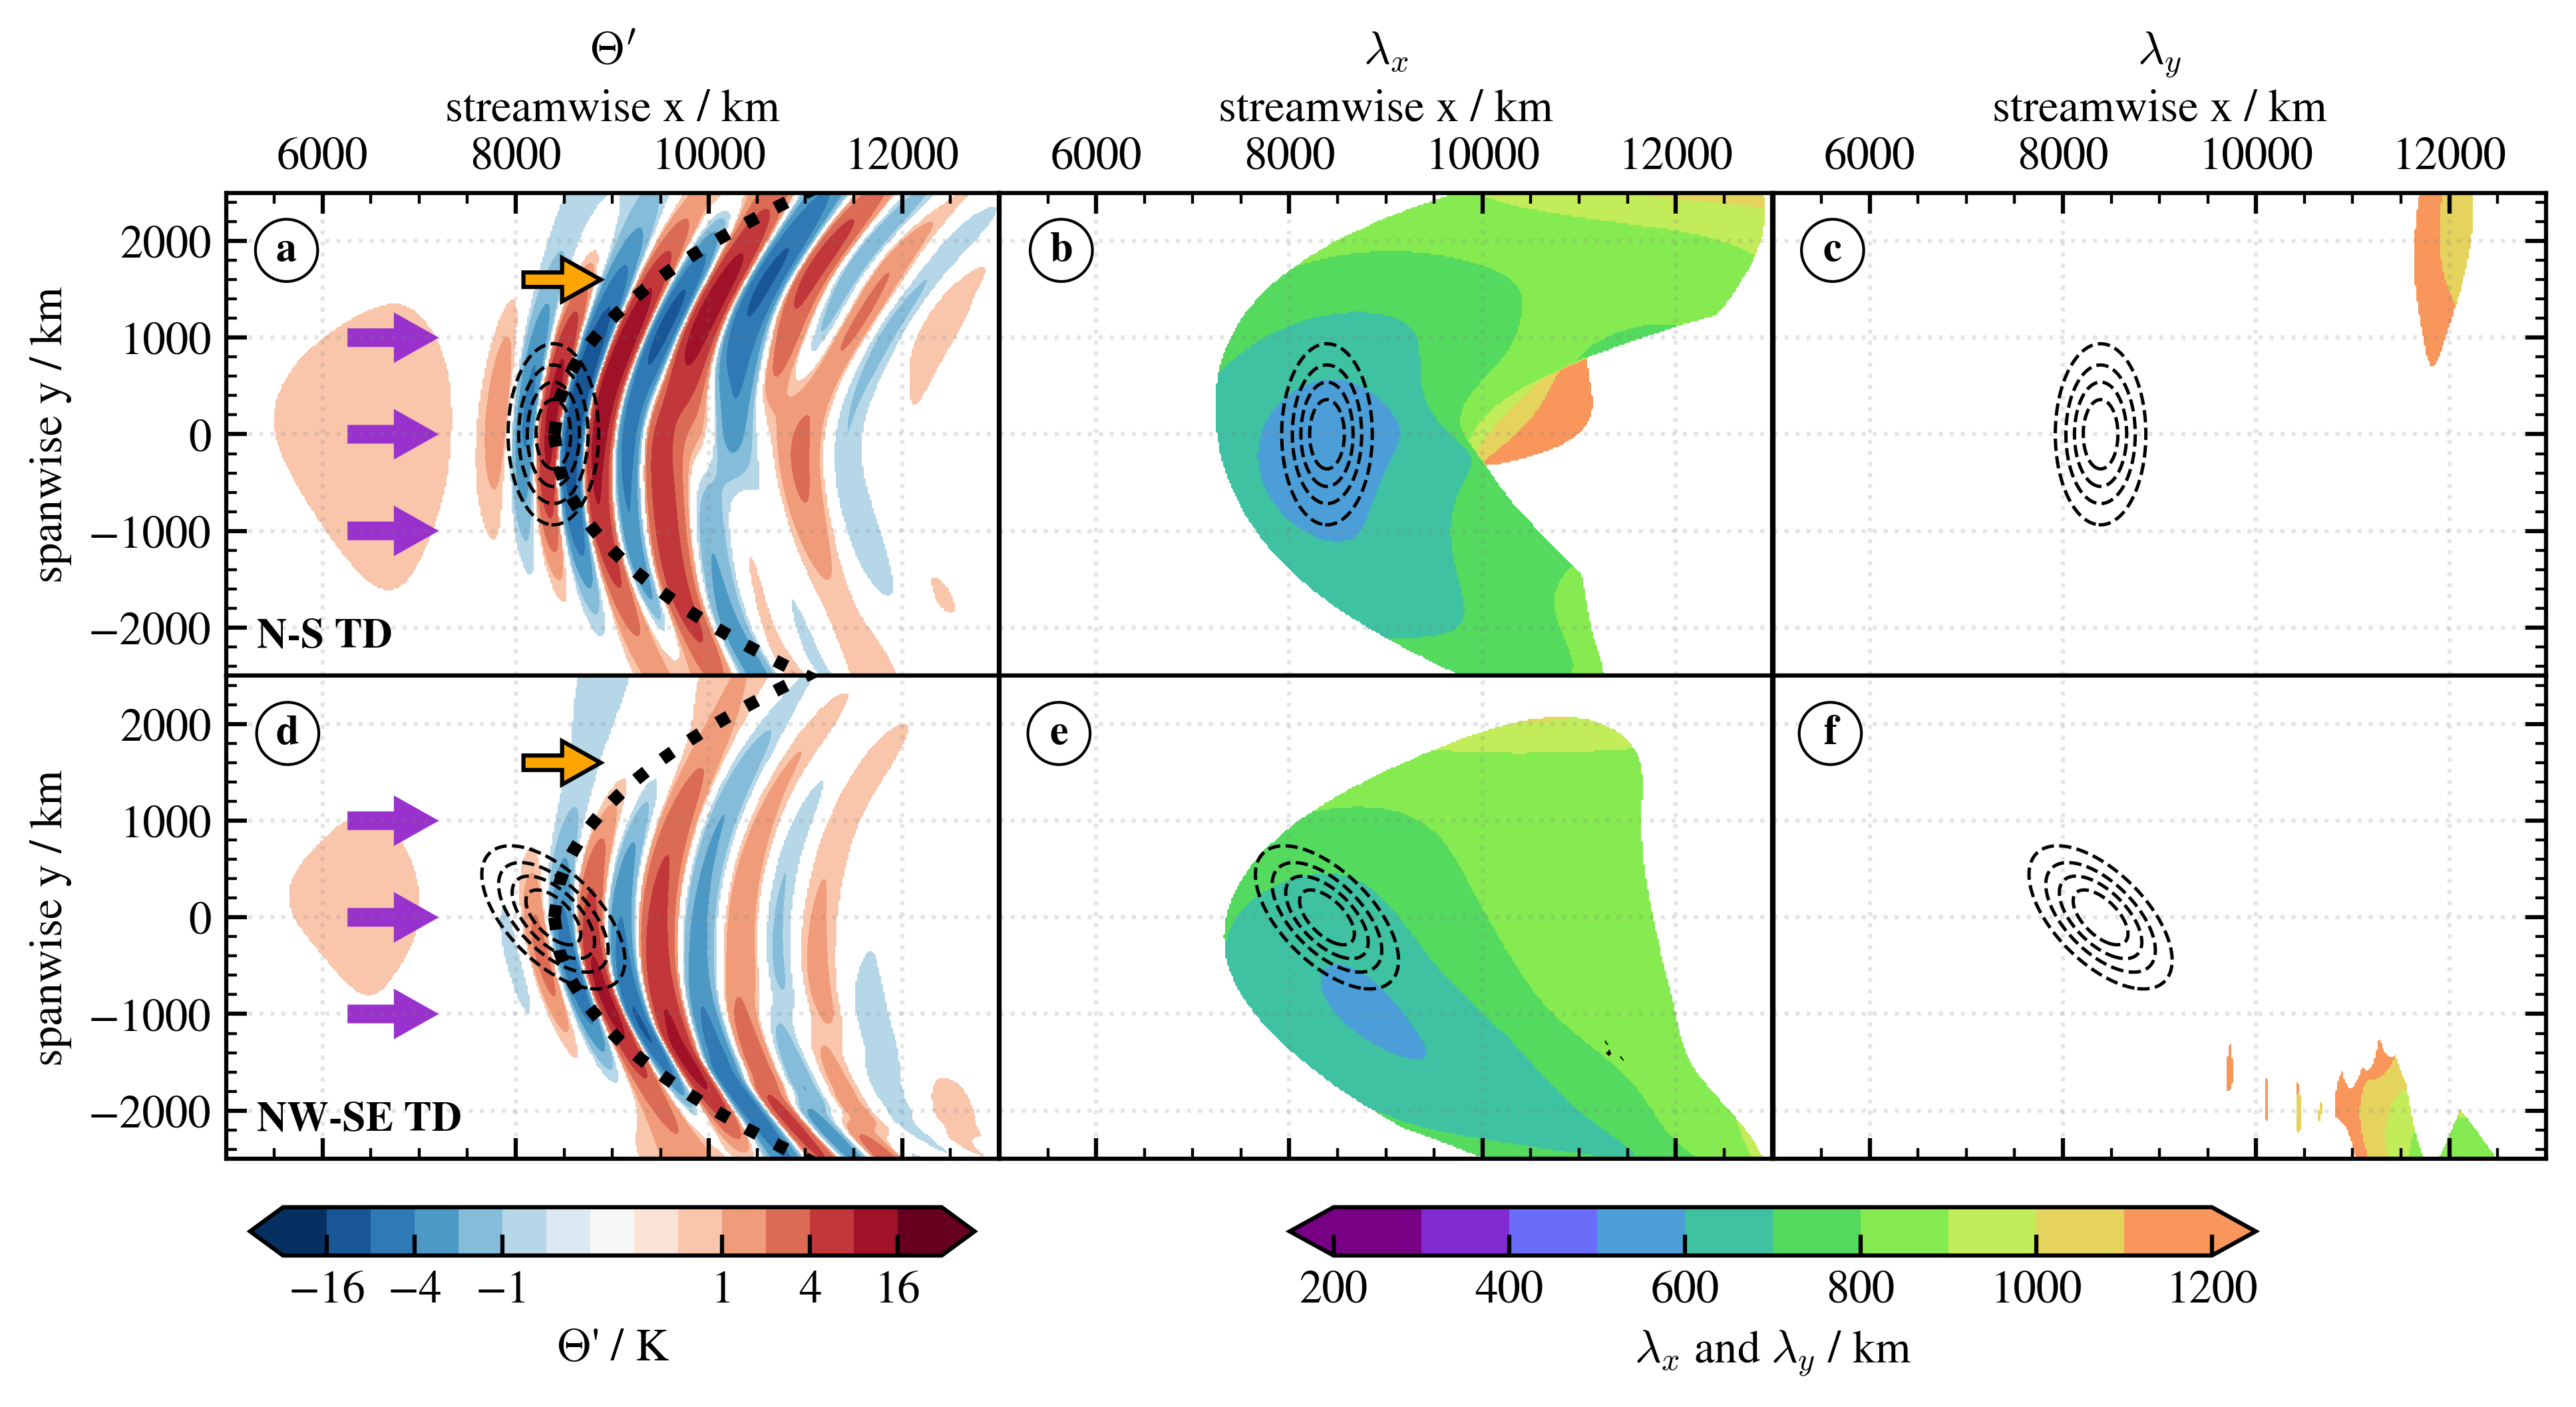
\includegraphics[width=0.99\textwidth]{figures_3D/waveletAna_overview_noShear.png}
    \caption{Horizontal cross-sections at \SI{40}{\kilo\meter} above the tropopause for two simulations with no meridional shear as indicated by the purple arrows. Shown are $\Theta$', $\lambda_x$ and $\lambda_y$ after \SI{72}{\hour}. Dominant wavelengths at each grid point are based on a 1D wavelet analysis in all three dimensions and values below the \SI{95}{\percent} confidence level (with respect to red noise) are left out. The dotted lines in (a) and (d) represent the U-shaped pattern (Equation (\ref{equ:smith_parabola})) of GW activity derived by \textcite[]{smith_linear_1980} for linear MWs above a circular Witch of Agnesi mountain in a non-rotating fluid. The first row (a,b and c) shows a simulation with a tropopause depression oriented north-south, the second row (d,e and f) shows a simulation with a tilted depression.}
    \label{fig:waveletAna_noShear}
    % in a barotropic environment
\end{figure*}
This first section can be seen as a transition from simulations of the previous chapter with no meridional variations of the tropopause depression and the background wind ($u_e(z)$) to simulations of the remaining chapter with meridional wind shear ($u_e(z,y)$) and an elliptical tropopause shape. Here, two simulations without meridional wind shear are presented for a tropopause depression where its depth varies spanwise in contrast to simulations of the preceding chapter. In this way, the effect of the depression's meridional shape on the GW propagation can be isolated and it is not superimposed by the effect of meridional wind gradients.

Horizontal cross-sections at $z=\SI{40}{\kilo\meter}$ and $t=\SI{72}{\hour}$ for both simulations are shown in Figure \ref{fig:waveletAna_noShear}. The background wind is similar to the yellow simulation in Figure \ref{fig:q3D_wind} with a $u_{PNJ,max}=\SI{100}{\meter\per\second}$ and no meridional gradients as indicated by the purple arrows in (a) and (d). In the upper simulation of Figure \ref{fig:waveletAna_noShear} (a,b and c), the zonal half width of the cosine tropopause depression is again $L_x=\SI{300}{\kilo\meter}$ and the meridional one is twice as wide with $L_y=\SI{600}{\kilo\meter}$. In the lower simulation (d,e and f) this tropopause depression is rotated horizontally by \SI{45}{\degree}, so the longer axis of the depression is oriented north-west to south-east (NW-SE). Dashed lines in Figure \ref{fig:waveletAna_noShear} outline the shape of the depression and clarify the orientation. \\
The observed GW pattern in the simulation with a north to south (N-S) oriented depression coincides with the theory of \textcite[]{smith_linear_1980}. The main GW activity aloft mimics a parabola (U-shape) that departs from the center and extends into the lee of the tropopause depression. \textcite[]{smith_linear_1980} neglected rotational effects and derived his linear solutions for GWs above an isolated circular Witch of Agnesi mountain (Equation (\ref{equ:agnesi})) and for a constant wind profile. He states that his results should be applicable to scales from 5 to \SI{50}{\kilo\meter}, but Figure \ref{fig:waveletAna_noShear} demonstrates that it is still a good approximation for variations from the idealized setup and for larger scales that are subject to rotational effects. The thick dotted lines in (a) and (d) represent the solution of Smith's parabola
\begin{equation}
    y^2 = \frac{L \, N}{U} z \, x
    \label{equ:smith_parabola}
\end{equation}
for $L=\SI{300}{\kilo\meter}$, $U=\SI{100}{\meter\per\second}$, $N=\SI{0.02}{\per\second}$ and $z=\SI{40}{\kilo\meter}$. The meridional asymmetry of the GW perturbations in (a) is caused by the Coriolis force with slightly stronger perturbations in the north (Coriolis frequency $f$ is negative in simulations to emulate the Southern Hemisphere), but the general picture in (a) fits to the U-shape described by \textcite[]{smith_linear_1980} for GWs aloft. Maximum temperature amplitudes are roughly one wavelength leeward of Smith's parabola. \\
In the idealized linear setup of \textcite[]{smith_linear_1980}, phase lines along the parabola always point back towards the GW source, so the wave's orientation changes proportional to the distance from the source region. In the simulation with a N-S oriented tropopause depression ((a),(b) and (c) in Figure \ref{fig:waveletAna_noShear}), this effect is weak but noticeable. (b) and (c) depict zonal ($\lambda_x$) and meridional ($\lambda_y$) wavelengths from a 1D wavelet analysis (Section \ref{sec:wavelet}) and, in particular, $\lambda_x$ increases along the parabola and indicates a turning of the horizontal wave vector. $\lambda_y$ is too large in the proximity of the tropopause fold (besides some values in the top right corner of (c)) and, in this context, phase lines rather point towards a leeward area of the fold and not towards its center, but this discrepancy is plausible and likely results from the elliptic (not circular) shape of the depression.

The effect of tilting the tropopause depression with respect to the zonal flow is apparent in (d),(e) and (f) of Figure \ref{fig:waveletAna_noShear}. A NW-SE oriented depression channels the GW activity southward, though the Coriolis effect counteracts. The shortest wavelengths are now located south of the depression (bluish colors in (e)) and, again, $\lambda_x$ increases along the parabola while values for $\lambda_y$ are only significant far south-east of the depression in (f). Phase lines along the parabola in (d) tend to point closer to the center of the depression compared to the first simulation in (a), because the difference between the streamwise and spanwise extend of the depression is decreased by the horizontal rotation.

Horizontal cross-sections of potential energy (E$_p$) and zonal and meridional momentum flux (MF) in Figure \ref{fig:waveletAna_noShear_mf} emphasize the southward channeling of GW activity for the NW-SE oriented depression. At \SI{40}{\kilo\meter} E$_p$, MF$_x$ and MF$_y$ decrease north of the depression and increase south of the depression with maximum absolute values again leeward of Smith's idealized parabola. For example, the maximum southward MF$_y$ at \SI{40}{\kilo\meter} in Figure \ref{fig:waveletAna_noShear_mf}f increased by \SI{165}{\percent} due to the rotation of the tropopause depression.

In summary, the meridional shape of an obstacle (e.g. a tropopause depression) significantly influences the propagation direction of excited GWs. Simply rotating the tropopause depression in the horizontal plane modified zonal and meridional momentum fluxes, and in the case of a NW-SE oriented depression in an environment without meridional wind shear, the southward momentum flux more than doubled. How this rotation influences the GWs in a more realistic scenario with meridional wind shear will be discussed in Section \ref{sec:3D_shape}.

% \cite[]{smith_linear_1980}
% $Fr=\frac{U}{h_m \, N} \approx 2$
% shall see that the small-amplitude theory describes the tendency of the flow to be diverted around the mountain but that this theory is valid only for large Froude number F
% All three of the qualitative features; the radial, outward tilting phase lines, the concentration of the disturbance along parabolas which widen with height, and the decay away from the mountain,
% along parabolas which widen with height z, and the decay away from the mountain, are evident 

% The obstacle feels closer to a circular shape for the wind""""
% deflected laterally!
% in the presence of gradients in meridional wind

%%% PNJ with meridional shear %%%
\section{The influence of meridional shear}
\label{sec:3D_shear}
Let us recall the equation for the temporal evolution of the meridional wavenumber from linear ray-tracing
\begin{equation}
    \frac{dl}{dt} = -(k \frac{\partial U}{\partial y} + l \frac{\partial V}{\partial y} + \frac{\beta f}{\hat{\omega}})
    \approx -k \frac{\partial U}{\partial y}
    \label{equ:meridionalRefraction2}
\end{equation}
mentioned in the introduction (e.g. \cite[]{dunkerton_inertiagravity_1984} or \cite[]{eckermann_ray-tracing_1992}). In our simulations $f$ is constant and the background flow is purely zonal, so $\beta=0$ and $\frac{\partial V}{\partial y}=0$ lead to the approximation in Equation (\ref{equ:meridionalRefraction2}). For conservative wave propagation and a stationary background flow $U$, the ground-based frequency $\omega$ is conserved along a ray ($\frac{d \omega}{d t} = 0$) and 
\begin{equation}
    \omega = k c_{P,x} + l c_{P,y} = \textrm{const.}
    \label{equ:const_omega}
\end{equation}
with $c_{P,x}$ and $c_{P,y}$ being the components of the ground-based horizontal phase speed (\cite[]{lighthill_waves_1978} and \cite[]{eckermann_ray-tracing_1992}). Therefore, modifications of $l$ due to the background shear (Equation (\ref{equ:meridionalRefraction2})) always imply a change of $k$ and a turning of the GW phase lines. Linear theory also shows that the direction of the horizontal wave vector ($k$,$l$) and of the intrinsic horizontal group velocity are equal for upward propagating GWs (\cite[]{sato_origins_2009}). Under the assumption of a purely zonal background flow the sign of $l$ is equal to that of the ground-based meridional group velocity and represents the direction of wave propagation.\\
The approximation on the right-hand side of Equation (\ref{equ:meridionalRefraction2}) shows two terms that are relevant for the generation of a meridional wave component $l$, the meridional shear $\frac{\partial U}{\partial y}$ and the zonal wavenumber $k$. Variations of the zonal wavenumber $k$ or wavelength $\lambda_x$ are closely related to the zonal shape of the tropopause depression and will be discussed in the next section. At first, this section focuses on meridional variations of the background wind.

\begin{figure*}[tbp]
    \centering
    \includegraphics[width=0.99\textwidth]{figures_3D/3D-th-referenceSim.png}
    \caption{The reference simulation of the entirely 3D simulations with meridional background wind shear. (a),(c) and (e) show horizontal cross-sections of $\Theta'$ at z=\SI{40}{\kilo\meter} for three timestamps. (b),(d) and (f) show corresponding meridional cross-sections \SI{900}{\kilo\meter} in the lee of the propagating tropopause fold. The position is also indicated in the horizontal cross-sections by the dashed black lines. The purple lines in (a),(c) and (e) refer to the location of the PNJ. Meridional cross-sections also show zonal wind $u$ (dashed lines) and isentropes (solid lines).}
    \label{fig:3D-reference}
\end{figure*}
\begin{figure*}[tbp]
    \centering
    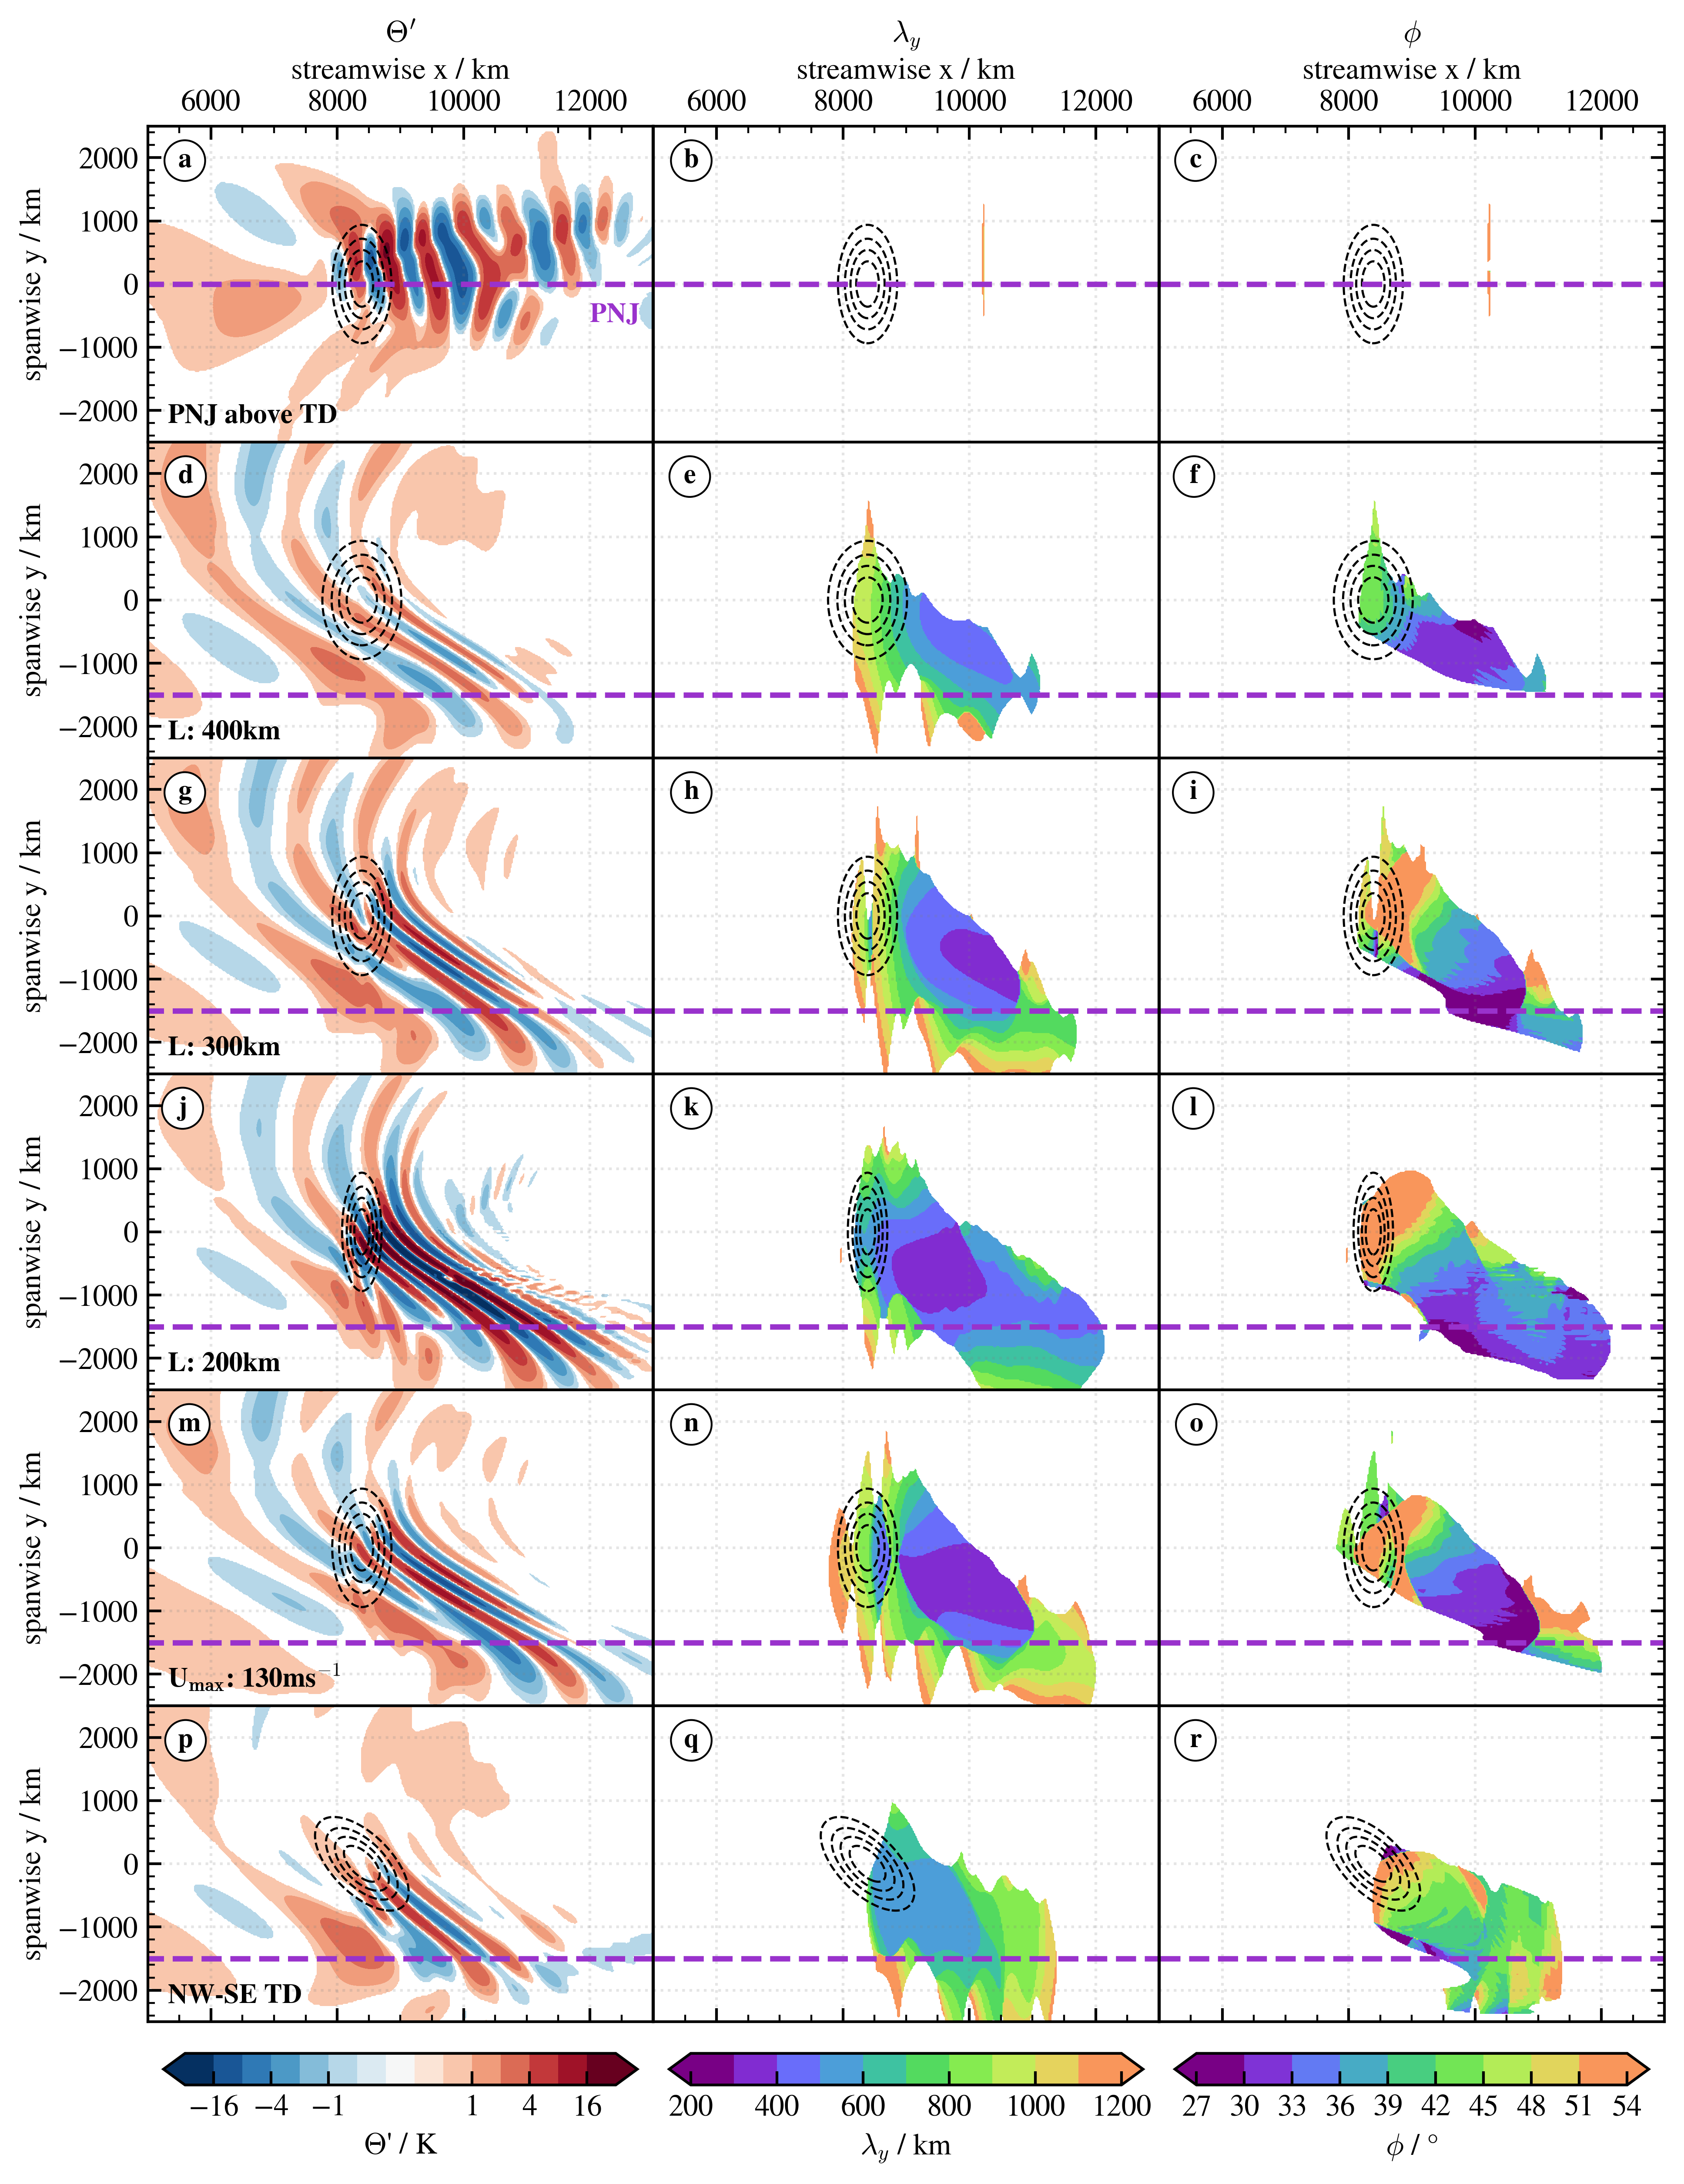
\includegraphics[width=0.96\textwidth]{figures_3D/waveletAna_angle.png}
    \caption{Similar to Figure \ref{fig:waveletAna_noShear}, but showing simulations with meridional wind shear as visualized in Figure \ref{fig:wind_profs}b. Here, $\lambda_y$ moved to the second column and the third column presents the angle $\phi=\arctan(\frac{\lambda_y}{\lambda_x})$ between the phase lines and the x-axis. Again, each row refers to a different simulation and the second and third column is based on a 1D wavelet analysis in each dimension. The corresponding zonal wavelength $\lambda_x$ and the vertical wavelength $\lambda_z$ are plotted in Figure \ref{fig:waveletAna_xz} in Appendix \ref{appA}. The third row ((g),(h) and (i)) is the reference simulation presented in Figure \ref{fig:3D-reference} and labels in each row describe the respective variation. The horizontal purple lines indicate the center of the PNJ.}
    % Hashed areas in the  below \SI{30}{\degree}. For clarification $\phi$ and $\lambda_z$ are plotted in Figure \ref{fig:waveletAna_angle} in Appendix \ref{appA}.
    % Hashed areas in the third column indicate vertical wavelengths larger than \SI{20}{\kilo\meter} at z=\SI{40}{\kilo\meter}.
    \label{fig:waveletAna}
    % between 6 and \SI{20}{\kilo\meter}
\end{figure*}
Figures \ref{fig:3D-reference} and \ref{fig:waveletAna} provide the basis for the following discussion. The first one shows the evolution of the reference simulation for the scenario with meridional wind shear ($u_e(z,y)$ as in Figure \ref{fig:wind_profs}b). The center of the PNJ is \SI{1500}{\kilo\meter} south of the tropopause depression centered at $y=0$, because this represents a common scenario above the Southern Ocean west and south of Australia with a PNJ at approximately \SI{60}{\degree S} and Rossby wave trains with tropopause folds further to the north between 30-\SI{55}{\degree S} (\cite[]{skerlak_tropopause_2015}). The 2D wind profile in the meridional cross-sections ((b),(d) and (f)) is the product of the vertical wind profile used in the previous section and a meridional distribution centered at $y=\SI{-1500}{\kilo\meter}$ (red curve in Figure \ref{fig:wind_profs}b which is also based on Equation (\ref{equ:wind-distribution})). As in the preceding section, the widths of the depression are $(L_x,L_y)=(\SI{300}{\kilo\meter},\SI{600}{\kilo\meter})$ and the tropopause propagates zonally with a constant speed $c_{tf}=\SI{13.88}{\meter\per\second}$.

In Figure \ref{fig:3D-reference} GWs excited above the tropopause depression are apparently refracted southward into the PNJ and develop a significant meridional wave vector component $l$, so phase lines in the horizontal cross-sections turn counterclockwise. The wavelet analysis in Figure \ref{fig:waveletAna} confirms this impression. The third row ((g),(h) and (i)) belongs to the reference simulation and, clearly, $\lambda_y$ is smaller south-east of the depression where the GW has propagated into the PNJ. In the same area, the angle $\phi=\arctan(\frac{\lambda_y}{\lambda_x})$ between the phase lines and the x-axis is also smaller and implies a rotation of the wave vector. The corresponding $\lambda_x$ is visualized in Figure \ref{fig:waveletAna_xz} in Appendix \ref{appA} and is larger close to the PNJ. \\
These observations are entirely consistent with linear ray-tracing theory and Equations (\ref{equ:meridionalRefraction2}) and (\ref{equ:const_omega}). MW-like GWs propagate against the background flow and imply a negative $k$. Moreover, the southward shift of the PNJ with respect to the GW source in the center of the domain leads to a negative $\frac{\partial U}{\partial y}$ north of the PNJ and hence $l$ increases in magnitude, but with a negative sign. A negative meridional wave vector component develops and the GW is refracted southward into the PNJ. It is clear that this process is not unlimited. As $l$ increases, $k$ decreases (Equation (\ref{equ:const_omega})) and starts to dampen the further development of a meridional wave component due to $\frac{\partial U}{\partial y}$ in Equation (\ref{equ:meridionalRefraction2}).

A PNJ centered above the tropopause depression as in (a),(b) and (c) of Figure \ref{fig:waveletAna} completely alters the GW pattern. Here, $\frac{\partial U}{\partial y}$ is negative in the north of the depression and positive in the south. GWs that propagate to the north (south) develop a negative (positive) $l$ and are refracted back towards the center of the domain. Again, GWs propagate towards the maximum wind speed of the PNJ, but in this scenario the generation of a meridional wave component $l$ is suppressed and phase lines stay more or less orthogonal to the zonal background flow.
% as depicted in (a) and (b) of Figure \ref{fig:waveletAna}

In the simulation of (m),(n) and (o) (row five of Figure \ref{fig:waveletAna}) the maximum wind speed of the PNJ is increased from $U_{PNJ,max}=\SI{100}{\meter\per\second}$ to $U_{PNJ,max}=\SI{130}{\meter\per\second}$. Signs for $k$ and $\frac{\partial U}{\partial y}$ are similar to the reference simulation, so GWs also propagate southward. However, the development of a negative $l$ and the corresponding turning of the wave is stronger, because the absolute value of $\frac{\partial U}{\partial y}$ is larger. Comparing (h) and (i) to (n) and (o) in Figure \ref{fig:waveletAna} supports this statement. $\lambda_y$ in (n) is generally smaller than in (h) and $\phi$ in (o) indicates a trend towards more horizontal phase lines with smaller $\lambda_y$ (wide purple area north of the PNJ), too. The stronger PNJ decreased the minimum angle $\phi$ derived from the wavelet analysis by \SI{2.7}{\degree} from \SI{24.6}{\degree} to \SI{21.9}{\degree}. \\
The stronger PNJ also increases energy fluxes and MF$_x$ and MF$_y$ visualized in the fifth row in Figure \ref{fig:waveletAna_mf}. For example, the maximum southward MF$_y$ in (o) is increased by \SI{75}{\percent} compared to the reference simulation in the third row.

We also note that GW phase lines in the horizontal cross-section at z=\SI{40}{\kilo\meter} (Figure \ref{fig:waveletAna}m) appear similar to the zonally elongated phase lines in the ERA5 data (Figure \ref{fig:RF25_era5_horizonal}) observed by \textcite[]{dornbrack_stratospheric_2022} and addressed in research question (R3). Strong winds in the upper stratosphere and the southward position of the PNJ seem to be necessary features to observe such a GW pattern. These conditions are likely in the Southern Hemisphere, and simulations in Figure \ref{fig:waveletAna} demonstrate that propagating tropopause depressions can excite GWs with zonally elongated phase lines. The influence of the tropopause shape in the presence of meridional wind shear is discussed in the next section.

% Another view on this refraction of GWs into the PNJ are critical levels... ??
% ground-based horizontal phase speed is always parallel to K 
% This lies the foundation for the following discussion.
% relative to the mean wind = intrinsic
% A = E/\omega$ = const.$  is the wave action 
% $ \omega = \hat{\omega} + k U = const.$ 
% beta = df/dy so beta plane approximation, usually also gradient of f changes on Earth
% trailing GWs 

\section{The influence of the tropopause shape in the context of meridional shear}
\label{sec:3D_shape}
%As stated in the previous section, 
The zonal wavenumber $k$ in Equation (\ref{equ:meridionalRefraction2}) is closely linked to the zonal width of the tropopause depression. A depression with a smaller width excites GWs with a smaller horizontal scale (larger $k$) and consequently, the growth of a meridional wave component $\frac{dl}{dt}$ in the presence of meridional wind shear is greater. The second (fourth) row of Figure \ref{fig:waveletAna} displays a simulation with a wider (narrower) tropopause depression as the reference simulation. Comparing these three simulations confirms the ray-tracing theory. The smaller the depression's zonal width $L_x$, the smaller $\lambda_x$ ((e),(h) and (k) in Figure \ref{fig:waveletAna_xz}) and the smaller $\lambda_y$ ((f),(i) and (l)in Figure \ref{fig:waveletAna}) in the upper stratosphere. In Chapter \ref{sec:resultsQ3D}, we also concluded that the GW activity in the stratosphere is inversely proportional to the width of the tropopause depression. Figure \ref{fig:waveletAna_mf} in Appendix \ref{appA} further substantiates this fact and emphasizes that the zonal ((e),(h) and (k)) and the meridional ((f),(i) and (l)) momentum flux increases for smaller depression widths. For example, maximum southward MF$_y$ at $\SI{40}{\kilo\meter}$ increased by a factor of 11 ($L_x$: $\SI{400}{\kilo\meter} \rightarrow \SI{300}{\kilo\meter}$) and by a factor of 7 ($L_x$: $\SI{300}{\kilo\meter} \rightarrow \SI{200}{\kilo\meter}$) for smaller $L_x$.   

A decreasing depression width implies decreasing GW scales and an increase of the zonal and meridional momentum flux, but does it also influence the orientation of the wave vector? In this context, we again refer to the angle $\phi$ at $\SI{40}{\kilo\meter}$ in the third column of Figure \ref{fig:waveletAna}. Though variations of the depression width are high between simulations, there is no clear trend of the ratio $\frac{\lambda_y}{\lambda_x}$ or the orientation of the wave vector ((f),(i) and (l)). All three simulations exhibit a similar pattern with rather spanwise oriented phase lines above and in the lee of the depression, and more streamwise oriented phase lines closer to the PNJ where $\frac{\partial U}{\partial y}$ increases. But a trend towards smaller $\phi$, as for the stronger PNJ in row 5 of Figure \ref{fig:waveletAna}, is not observable.

\begin{figure*}[t]
    \centering
    \includegraphics[width=0.99\textwidth]{figures_3D/3D-EF-MF.png}
    \caption{Similar cross-sections as Figure \ref{fig:3D-reference} with horizontal cross-sections at z=\SI{40}{\kilo\meter} in (a) and (c) and meridional cross-sections in (b) and (d) for x=\SI{9400}{\kilo\meter} showing meridional momentum flux MF$_y$ instead of $\Theta'$. The first row is again the 3D "reference" simulation at $t=\SI{72}{\hour}$, the second row is a simulation with identical settings, but a NW-SE oriented tropopause depression. In other words, the depression is rotated horizontally by 45°. Black arrows in (a) and (c) illustrate the direction and relative value of the horizontal energy flux \textbf{EF}. The reference simulation is the third row and the simulation with a rotated depression is represented by the last row in Figure \ref{fig:waveletAna}.}
    \label{fig:3D-MFy}
\end{figure*}
The last row in Figure \ref{fig:waveletAna} presents a simulation with a rotated tropopause depression as in Section \ref{sec:3D_noshear}, but in the presence of meridional wind shear. Interestingly, $\lambda_y$ and $\phi$ are larger for the NW-SE oriented depression, so rotating the depression reduces the development of $l$ and zonally elongated phase lines. Furthermore, the meridional momentum flux MF$_y$ in Figure \ref{fig:3D-MFy} is lower for the simulation with a NW-SE oriented depression in (c) and (d) compared to a N-S oriented depression with an identical size in (a) and (b). It seems counterintuitive because in the no-shear case of Section \ref{sec:3D_noshear}, the NW-SE oriented depression slightly favors the development of a meridional wave vector component and substantially increases the maximum southward MF$_y$ by more than \SI{150}{\percent}. However, the wider width in the direction of the background flow reduces $k$ and the growth of $l$ and, therefore, constrains the refraction and meridional propagation of the GW due to Equation (\ref{equ:meridionalRefraction2}). Instead of increasing MF$_y$, the rotation of the depression more than halves the maximum southward MF$_y$. It is reduced by \SI{56}{\percent}.\\
Vectors of the horizontal energy flux \textbf{EF} in (a) and (c) emphasize the southward propagation of the GWs into the PNJ and the intrinsic propagation against the prevailing wind for both simulations, but again, \textbf{EF} is greater for the N-S oriented depression.

Overall, the meridional momentum and energy fluxes increase for smaller zonal widths of the tropopause depression, but $\phi$ or the zonally elongated phase line pattern in the upper stratosphere is not directly sensitive to the depression's zonal width. On the other hand, $\phi$ seems to be linked to the depression's orientation, because a NW-SE oriented depression results in a larger angle $\phi$ between the phase lines and the x-axis. This might be linked to its larger width in the direction of the background flow, but additional factors have to be relevant, too, because we generally conclude that $\phi$ is not sensitive to the zonal width from the simulations in rows 2-4 in Figure \ref{fig:waveletAna}.

% general statement on momentum fluxes larger for smaller scale GWs
%
\section{Summary and answer to research question (R2) and (R3)}
\label{sec:3D_summary}
This chapter mainly presented 3D simulations of the stratosphere with identical resolutions in streamwise and spanwise direction, with a meridionally varying lower boundary (tropopause) and with vertical and meridional gradients in the zonal background flow. It is the most realistic setup within the framework of this thesis and only a coupling of tropospheric and stratospheric airflows with a baroclinic instability at tropopause level and a PNJ in the upper stratosphere would be closer to reality. \\
As an extension to the 2D sensitivity study in Chapter \ref{sec:resultsQ3D}, this chapter focused on the sensitivity with respect to meridional properties of the tropopause and stratosphere and addressed the second research question.
\begin{tcolorbox}[]
    (R2) How sensitive are NOGWs from propagating tropopause depressions to the depression's 3D shape and meridional variations of the stratospheric airflow?
\end{tcolorbox}
In the context of no meridional wind shear (Section \ref{sec:3D_noshear}), the orientation of the tropopause depression can significantly alter the GW activity and channel GWs in one lateral direction. Tilting the depression with respect to the incoming flow increases the meridional propagation of GWs and more than doubles MF$_y$ though the wave vector is only marginally modified. In the presence of meridional wind shear, rotating the depression has the opposite effect and decreases meridional momentum and energy fluxes (MF$_y$ is reduced by more than \SI{50}{\percent}), because the depression's zonal width increases. This is consistent with the conclusion on the depression's zonal width in Chapter \ref{sec:resultsQ3D}. In summary, meridional momentum and energy fluxes in the upper stratosphere
\begin{itemize}
    \item are inversely proportional to the zonal width of the tropopause depression and MF$_y$ increases by a factor of 7-11 when reducing the zonal half width $L_x$ by \SI{100}{\kilo\meter}.
    \item decrease for a horizontally rotated tropopause depression and MF$_y$ is reduced by more than \SI{50}{\percent} in the presence of meridional wind shear (Figure \ref{fig:3D-MFy}).
    \item are proportional to the strength (wind speed) of the PNJ and MF$_y$ increases by \SI{75}{\percent} when increasing the $U_{PNJ,max}$ by \SI{30}{\meter\per\second}.
    \item are highly dependent on the relative meridional position of the PNJ. A PNJ directly above the depression minimizes the meridional propagation of GWs.
\end{itemize}
This chapter also focused on answering the third research question.
\begin{tcolorbox}[]
    (R3) Can NOGWs above propagating tropopause depressions explain the zonally elongated phase lines in ERA5 above the Southern Ocean?
    % the proposed excitation mechanism for 
    % the zonally elongated phase lines in the horizontal cross-sections of Figure \ref{fig:RF25_era5_horizonal}. 
    % long vertical wave lengths in vertical cross-section and elongated phase line in horizontal
    % Address vertical cross-section in introduction
\end{tcolorbox}
It refers to the zonally elongated phase lines in the horizontal cross-sections of Figure \ref{fig:RF25_era5_horizonal} observed by \textcite[]{dornbrack_stratospheric_2022}. At first, Section \ref{sec:3D_noshear} demonstrated that the orientation of the tropopause depression alone can not produce a comparable GW pattern to Figure \ref{fig:RF25_era5_horizonal} and the wave vector remains almost parallel to the zonal flow. By contrast, the meridional wind shear introduced in Section \ref{sec:3D_shear} can significantly alter the orientation of the wave vector and we conclude that a very strong PNJ located in the south of a tropopause depression leads to zonally elongated phase lines in the upper stratosphere similar to the appearance of GWs in Figure \ref{fig:RF25_era5_horizonal}. So NOGWs above propagating depressions could explain the GW structures in the upper stratosphere above the Southern Ocean. \\
The zonal width of the tropopause depression only influences momentum and energy fluxes in the context of changing scales, but it does not seem to alter the orientation of the wave vector. On the contrary, a horizontal rotation of the depression has a counterintuitive effect and leads to a larger angle $\phi$ between the phase lines and the x-axis. An increasing width in the direction of the incoming flow dampens the development of $l$, but it can not fully explain this phenomenon.   

It could be educational to investigate additional variations of the PNJ's meridional position on the angle $\phi$. Potentially, a PNJ closer to the tropopause depression (at for example $y=\SI{-750}{\kilo\meter}$) results in a smaller angle $\phi$.

%These results provide ad- ditional evidence of a widespread oblique propagation ef- fect, described in an increasing number of studies (Watanabe et al., 2008; Wu and Eckermann, 2008; Preusse et al., 2009; Sato et al., 2009, 2012; Ern et al., 2011; Kalisch et al., 2014; Hindley et al., 2015; Alexander et al., 2016; Ehard et al., 2017). 

% Motivated by the work of   Figure \ref{fig:RF25_era5_vertical}
% Phase lines in vertical cross-section triggered the analogy to MWs